\beginsong{Abends treten Elche}[
    wuw={Heinrich Eichen, Gerd Lascheit}, 
    jahr={1931}, 
    bo={3}, 
    pfii={6}, 
    pfiii={33}, 
    gruen={102}, 
    siru={2},
    tonspur={138},
]

\beginverse
\endverse
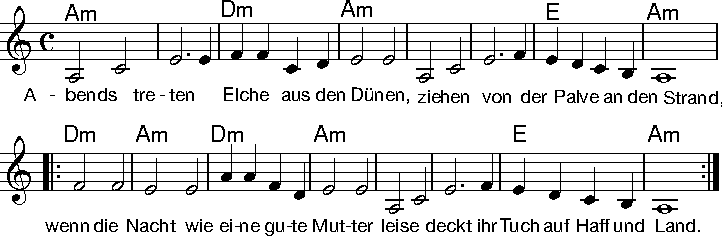
\includegraphics[draft=false, width=1\textwidth]{Noten/Lied002.pdf}

\beginverse
\[Am]Ruhig trinken \[Dm]sie vom großen \[Am]Wasser, 
darin Sterne \[E]wie am Himmel \[Am]steh'n.
\lrep \[Dm]Und sie heben ihre starken \[Am]Köpfe 
lautlos in des \[E]Sommerwindes \[Am]Weh'n. \rrep
\endverse

\beginverse
^Langsam schreiten ^wieder sie von ^dannen, 
Tiere einer ^längst vergang'^nen Zeit. 
\lrep ^Und sie schwinden in der Ferne ^Nebel 
wie im hohen ^Tor der Ewig^keit. \rrep
\endverse


\endsong
\beginscripture{}
Das Lied war in der ostpreußischen Bevölkerung - auch nach der Flucht vieler vor der Roten Armee 1945 in den Westen des Reiches - sehr beliebt.
\endscripture
